\section{Data}
\label{sec:data}

We explore the behavior of the metrics on mock classifications with well-understood weaknesses as well as realistic mock classifications from past challenges.
Data is in the form of catalogs of posterior probability vectors $p(m \mid d)$ over $M$ classes $m$ conditioned on the observed lightcurve $d$, with each probability vector normalized to sum to unity.\footnote{Throughout the paper, ```data'' always refers to classification results, not lightcurves; no \plasticc\ lightcurves were simulated, viewed, or classified in the preparation of this paper.}
% We introduce the convention that the $M^{\mathrm{th}}$ class is designated ``other'' to encompass never-before-seen classes.
We introduce the confusion matrix $\mathbb{C}$, an $M\times M$ dimensional table of empirical probabilities $p(m \mid m')$ traditionally calculated from deterministic classification point estimates with knowledge of the true classes $m'$.
Though probabilistic classifications are not truly compatible with the confusion matrix, we use it as a middle ground to develop intuition from conceptually familiar deterministic classifications.

\subsection{Mock classifications}
\label{sec:mockdata}

The test cases of this section are devised to confirm that our metric aligns with our intuitive understanding of what constitutes a good classifier, that it should not reward classifications suffering from the most concerning error properties, which we will refer to as \textit{systematics} throughout the paper.
We consider a situation with $M=13$ classes
% (nominally $12$ with one designated as ``other,'' meaning not represe) and
with a lognormal distribution of the number $N_{m}$ of members of each class.

We present eight mock classifiers whose systematics are encapsulated by their confusion matrix $\mathbb{C}$.
Each classifier derives classification posteriors $p(m \mid m')$ based on the true classes as a proxy for the information contained in the lightcurves, which we hope to recover.
The posterior probability vector for a given object is a perturbation of the row of the confusion matrix corresponding to its true class, with a perturbation factor of $\delta=0.1$, following
\begin{eqnarray}
  \label{eq:cmtoprob}
  p(m \mid m') &=& \mathbb{C}_{m'} + \delta\vec{\epsilon},
\end{eqnarray}
where the perturbation vector $\vec{\epsilon}$ has components drawn from a half-Cauchy distribution
\begin{eqnarray}
  \label{eq:cauchy}
  f(x) &=& \frac{2}{\delta\pi} \left(1+\left(\frac{x+x_{0}}{\delta}\right)^{2}\right)^{-1}
\end{eqnarray}
with $x_{0}=0$.
% \aim{[Rahul: Might be good to have a plot of the pdf when x0 takes values close to 0., something like 0.4, 0.8 and close to 1.0]}

Figure~\ref{fig:mock_cm} shows the confusion matrices corresponding to each systematic considered.
For each case, we address:
\begin{enumerate}
  \item What defines this systematic?
  \item When has this systematic been observed before?
  \item What are our expectations for this systematic's effect on metric behavior?
\end{enumerate}

%It might be good to have a sequential color bar, It would seem that the green in Perfect should correspond to lower values than the green in agnostic, and I think it is true, but hard to see in the color bar because of the colormap choice, It might be good to match the subsections to the plots. I am also not sure if the description of the subsumed classifiers is correct, it seems like a one to many sense is missing in the description. Finally, why is the tunnel vision correlation vertical?]}
\begin{figure*}
	\begin{center}
    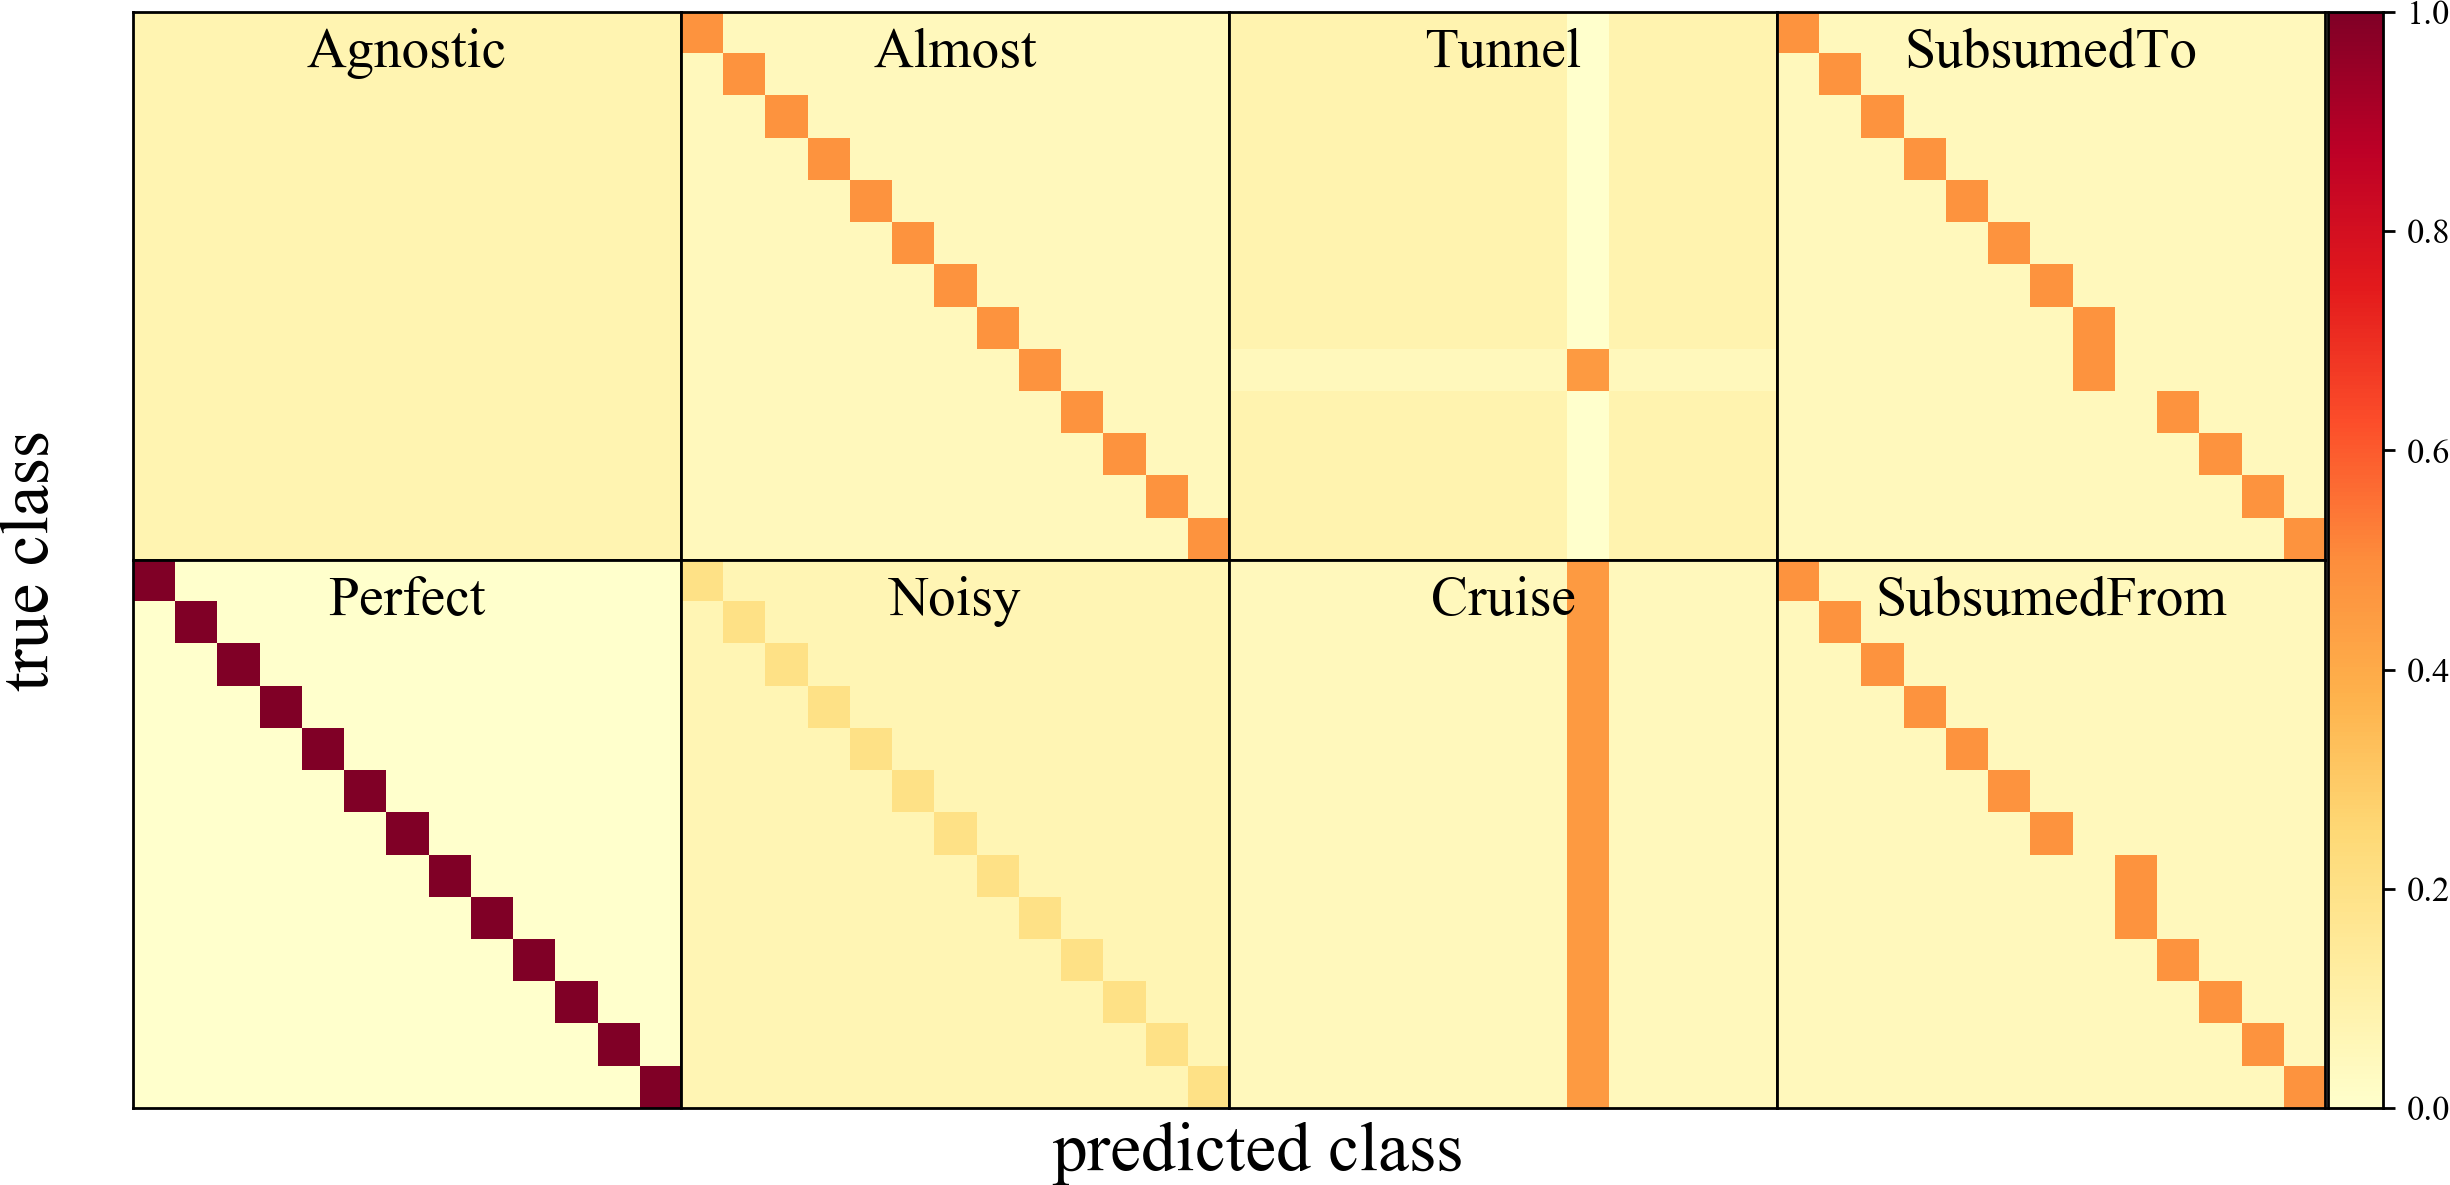
\includegraphics[width=0.8\textwidth]{./fig/all_sim_cm.png}
		\caption{Confusion matrices for eight mock classifiers.
    leftmost top: uncertain classification,
    leftmost bottom: perfect classifications,
    left-center top: almost perfect classification,
    left-center bottom: unbiased classifications,
    right-center top: perfect classification (type 1 and type 2 errors) for one class and uniform for all others,
    right-center bottom: assigning all objects the same class,
    rightmost top: consistently assign one class to another,
    rightmost bottom: consistently assign another class to one class}
		\label{fig:mock_cm}
	\end{center}
\end{figure*}

\subsubsection{Uncertain classification}
\label{sec:uncertaindata}

An entirely uniform confusion matrix would correspond to uniform random guesses for deterministic classification, but the probability vectors drawn from it are more nuanced.
In accordance with Equation~\ref{eq:cmtoprob}, the probability vectors are perturbations away from a  uniform distribution across all classes.
The peak values of these probability vectors will correspond to uniform random classifications, however, with $p(m' \mid d)\approx M_{\mathrm{classes}}^{-1}$.
We can consider the ``uncertain'' classifier as an experimental control for the worst possible classifier, noting that if classifications were anticorrelated with true classes, the experimenter would simply relabel them to improve performance.

\subsubsection{Accurate classification}
\label{sec:accuratedata}

The ``perfect'' classifier has a diagonal confusion matrix, which would correspond to deterministic classifications that are always correct.
In terms of probabilistic classifications, a perfect result would be a probability vector with 1 for the true class and 0 for all other classes.
Due to our addition of perturbing random variables, the probability vectors drawn from the perfectly diagonal confusion matrix are randomly perturbed away from perfect classifications by the small factor $\delta$, but the class with maximum probability is almost always still the true class, to the tune of $p(m' \mid d)\approx0.96$ with our choice of $\delta$.
This case is also a control, in that \plasticc\ would not be necessary if we believed the perfect classifier were realistically achievable.

In addition to a perfect classifier, we test linear combinations of the perfect and uncertain classifiers where the contribution of the perfect classifier is greater that of the uncertain classifier by a factor of $s$.
Deterministic classifications drawn from such a confusion matrix would be correct $s$ times as often as they are wrong, and the incorrect guesses would be uncorrelated across classes.
The probability vectors drawn from such confusion matrices would have some variability but still mostly have their peak value at the truth.
We consider the case of the ``almost perfect'' classifier with $s=4$ and the ``noisy'' classifier with $s=2$, which correspond to $p(m' \mid d)\approx0.82$ and $p(m' \mid d)\approx0.62$ respectively.
We expect that the response to variation in $s$ may differ across metrics.

When a classifier has differing levels of accuracy for each class, it can be considered a form of systematic.
An extreme example of such a classifier could be one with perfect classification performance on one class and uncertain classification on all others; its confusion matrix would be uniform except for one row, which would take a value of unity on the diagonal and zero elsewhere.
\aim{[Rahul: While it is clear that we don't want to reward a tunnel vision classifier, perhaps this should be rephrased. I think we want to state that this is our active decision: due to our diverse needs, we don't want to reward such a classifier, but calling it a foremost concern sounds like something could go wrong with our metric]}
This classifier suffers from ``tunnel vision'' and would correspond to one of the foremost concerns about the metric for \plasticc.
While such classifiers have value, they are not appropriate for a challenge serving diverse science goals, so the tunnel vision classifier is a major concern.

\subsection{Inaccurate classification}
\label{sec:inaccuratedata}

Inaccurate classification in the context of a deterministic classifier is self-explanatory.
If a classifier is systematically inaccurate, its confusion matrix would have significant probability on off-diagonal elements.
We model inaccurate probabilistic classifications of class $m'$ by using the row of the confusion matrix corresponding to class $\tilde{m}$ as the basis for the perturbed probability vector.
Class $m'$ is said to be ``subsumed'' by class $\tilde{m}$ for such a classifier.

It is possible that the \plasticc\ classes will be subtypes of broader classes, as identifying classifiers that can distinguish between subtypes is especially relevant when the subtypes have wholly different science applications.
For example, SN Ia and SN Ibc are challenging to distinguish, and the former often subsumes the latter, an effect that can be exacerbated by underrepresentation of SN Ibc in available training sets.
However, using SN Ibc in the traditional cosmology analysis done with SN Ia can bias estimates of the cosmological parameters, so the distinction is critical.
We would like to ensure that the \plasticc\ metric

An extreme case of inaccurate classification is to classify all objects as the most common class, a particular concern for \plasticc.
For our purposes, it matters not whether the subsuming class is actually the most common or only the most common in the training set.
Such a ``cruise control'' classifier could be especially dangerous to \plasticc's goal of identifying objects belonging to extremely rare classes, particularly if the metric weights all objects equally.
Though we defend against this systematic by employing per-class weights, described in Section~\ref{sec:weights}, we nonetheless examine its impact under other plausible weighting schemes.

% \subsubsection{Combination of systematics}
% \label{sec:combo}
%
% \begin{figure}
% 	\begin{center}
% 		% 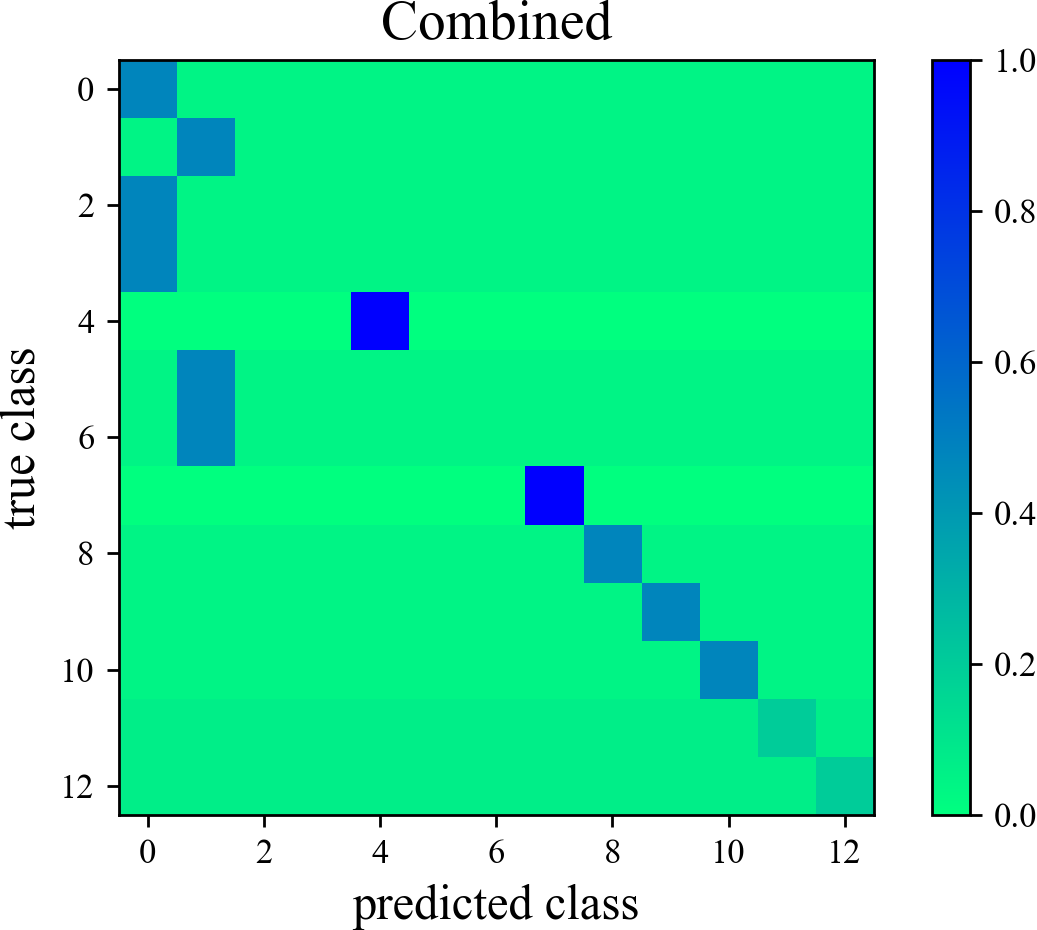
\includegraphics[width=0.45\textwidth]{./fig/Combined.png}
% 		\caption{}
% 		\label{fig:combo_cm}
% 	\end{center}
% \end{figure}

\subsection{Representative classifications}
\label{sec:realdata}
%\aim{This would be more meaningful if we were given the confusion matrices of actual submissions to \snphotcc\ and then checked whether the \plasticc\ metric would have designated a different winner.
%Also, it may be more interpretable if we instead use Ashish's confusion matrices that have more classes.
%As an alternative, however, Michelle Lochner has volunteered to write more about the representative classifications presented in this section as is.}

Classification problems in astronomy have historically focused on separating a heterogenous population into a limited number of subclasses \citep{kessler_results_2010}, with the focus or goal being to identify one particular type of object.

% In the Supernova Photometric Classification Challenge (SNPhotCC), the metric for deciding on who `won' the challenge was determined as a ratio of the efficiency of Type Ia classification and a `pseudo purity' factor, and a penalty for false-flagging (which is related to the cost of following up an object spectroscopically that is not a SNIa).
% The figure of merit was given by:
%
% \begin{eqnarray}
%   \label{eq:snphotcc}
% \mathcal{C}_{FOM-Ia} &\equiv& \frac{1}{\mathcal{N}_{Ia}^{TOT}}\times \frac{(N_{Ia}^{\mathrm{true}})^2}{N_{Ia}^\mathrm{true}+W_{Ia}^\mathrm{false}N_{Ia}^\mathrm{false}}
% \end{eqnarray}
% %\aim{Renee Hlozek will write the descriptions of these datasets.}
%
% The above reduces to $\mathcal{C}_{FOM-Ia}  = \epsilon_{Ia} + PP_{Ia},$ the efficiency and pseudopurity, which can be interpreted as the traditional purity factor in the limit that the weight $W_{Ia}^\mathrm{false} = 1$.
% For the SNPhotCC the false penalty was related to the size of the spectroscopic subsample as roughly $W_{Ia}^\mathrm{false} = 1 + \epsilon_{spec}^{-1} \gg 1$ but the conservative limit of $W_{Ia}^\mathrm{false} = 3$ was chosen to penalize wasted spectroscopic time over rejected SNe.
%
% For future challenges, a more balanced metric can be used to ensure correct classifications across the range of objects, without focusing or highlighting a specific object as above.
% Furthermore,

In response to the SNPhotCC, a range of classifications approaches were submitted, namely $\chi^{2}$ fits of the SN data to publicly available templates \citep[see the][templates,]{2002PASP..114..803N}, identification with the SiFTO light curve fitter \citep{2008ApJ...681..482C} through the fitted values of the stretch, colour and also the $\chi^{2}$ of the fit for Ia fits, and a linear slope to magnitudes per day was used for the non-Ia sample.
Other groups constructed a Hubble diagram from the training data, and used the residuals away from that Hubble diagram as a criterion for classification in the test data. Still other groups performed classification by reducing the dimensionality of the light curves (the so-called InCA approach).
A general light curve shape (rather than one motivated by the physical differences between SNeIa and core collapse SNe) was assumed by some competitors and then a kernel density estimation was performed over the fit parameters, with various approaches employed including boosting over the feature space.

Machine learning was also eployed over the reduced data set of light-curve slopes (in magnitudes per day) as above to produce a predictive model for the training data. For more information on these methods and their success within the SNPhotCC, we refer the reader to \cite{kessler_results_2010}.

The above approaches vary between very physically motivated and \textbf{template based} (and also prone to bias given non-representativity of the test data) and agnostic and based on decomposition of the light curves into \textbf{generic features} (but also making use of less information in the classifications).
In figure~\ref{fig:snphotcc_cm} we show a range of classification approaches over the wavelet (feature) space (top row) and using templates (bottom row).

After the SNPhotCC was complete, the data were used to test a suite of machine learning methods of classification. We consider one such compilation of methods, as presented in \cite{lochner_photometric_2016}. These classification algorithms include a wavelet decomposition of the spectra to construct the features over which to classify \citep{2011MNRAS.414.1987N} and template-based classification procedures \citep{2011ApJ...738..162S}, each paired with Boosted Random Forest, K-Nearest Neighbors, Naive Bayes, and Support Vector Machine machine learning algorithms. While the complexity of entries to the SNPhotCC was greater than this subset, this provides a useful comparison set over which to assess the performance of the approaches under our metric scheme.
\begin{figure*}
	\begin{center}
    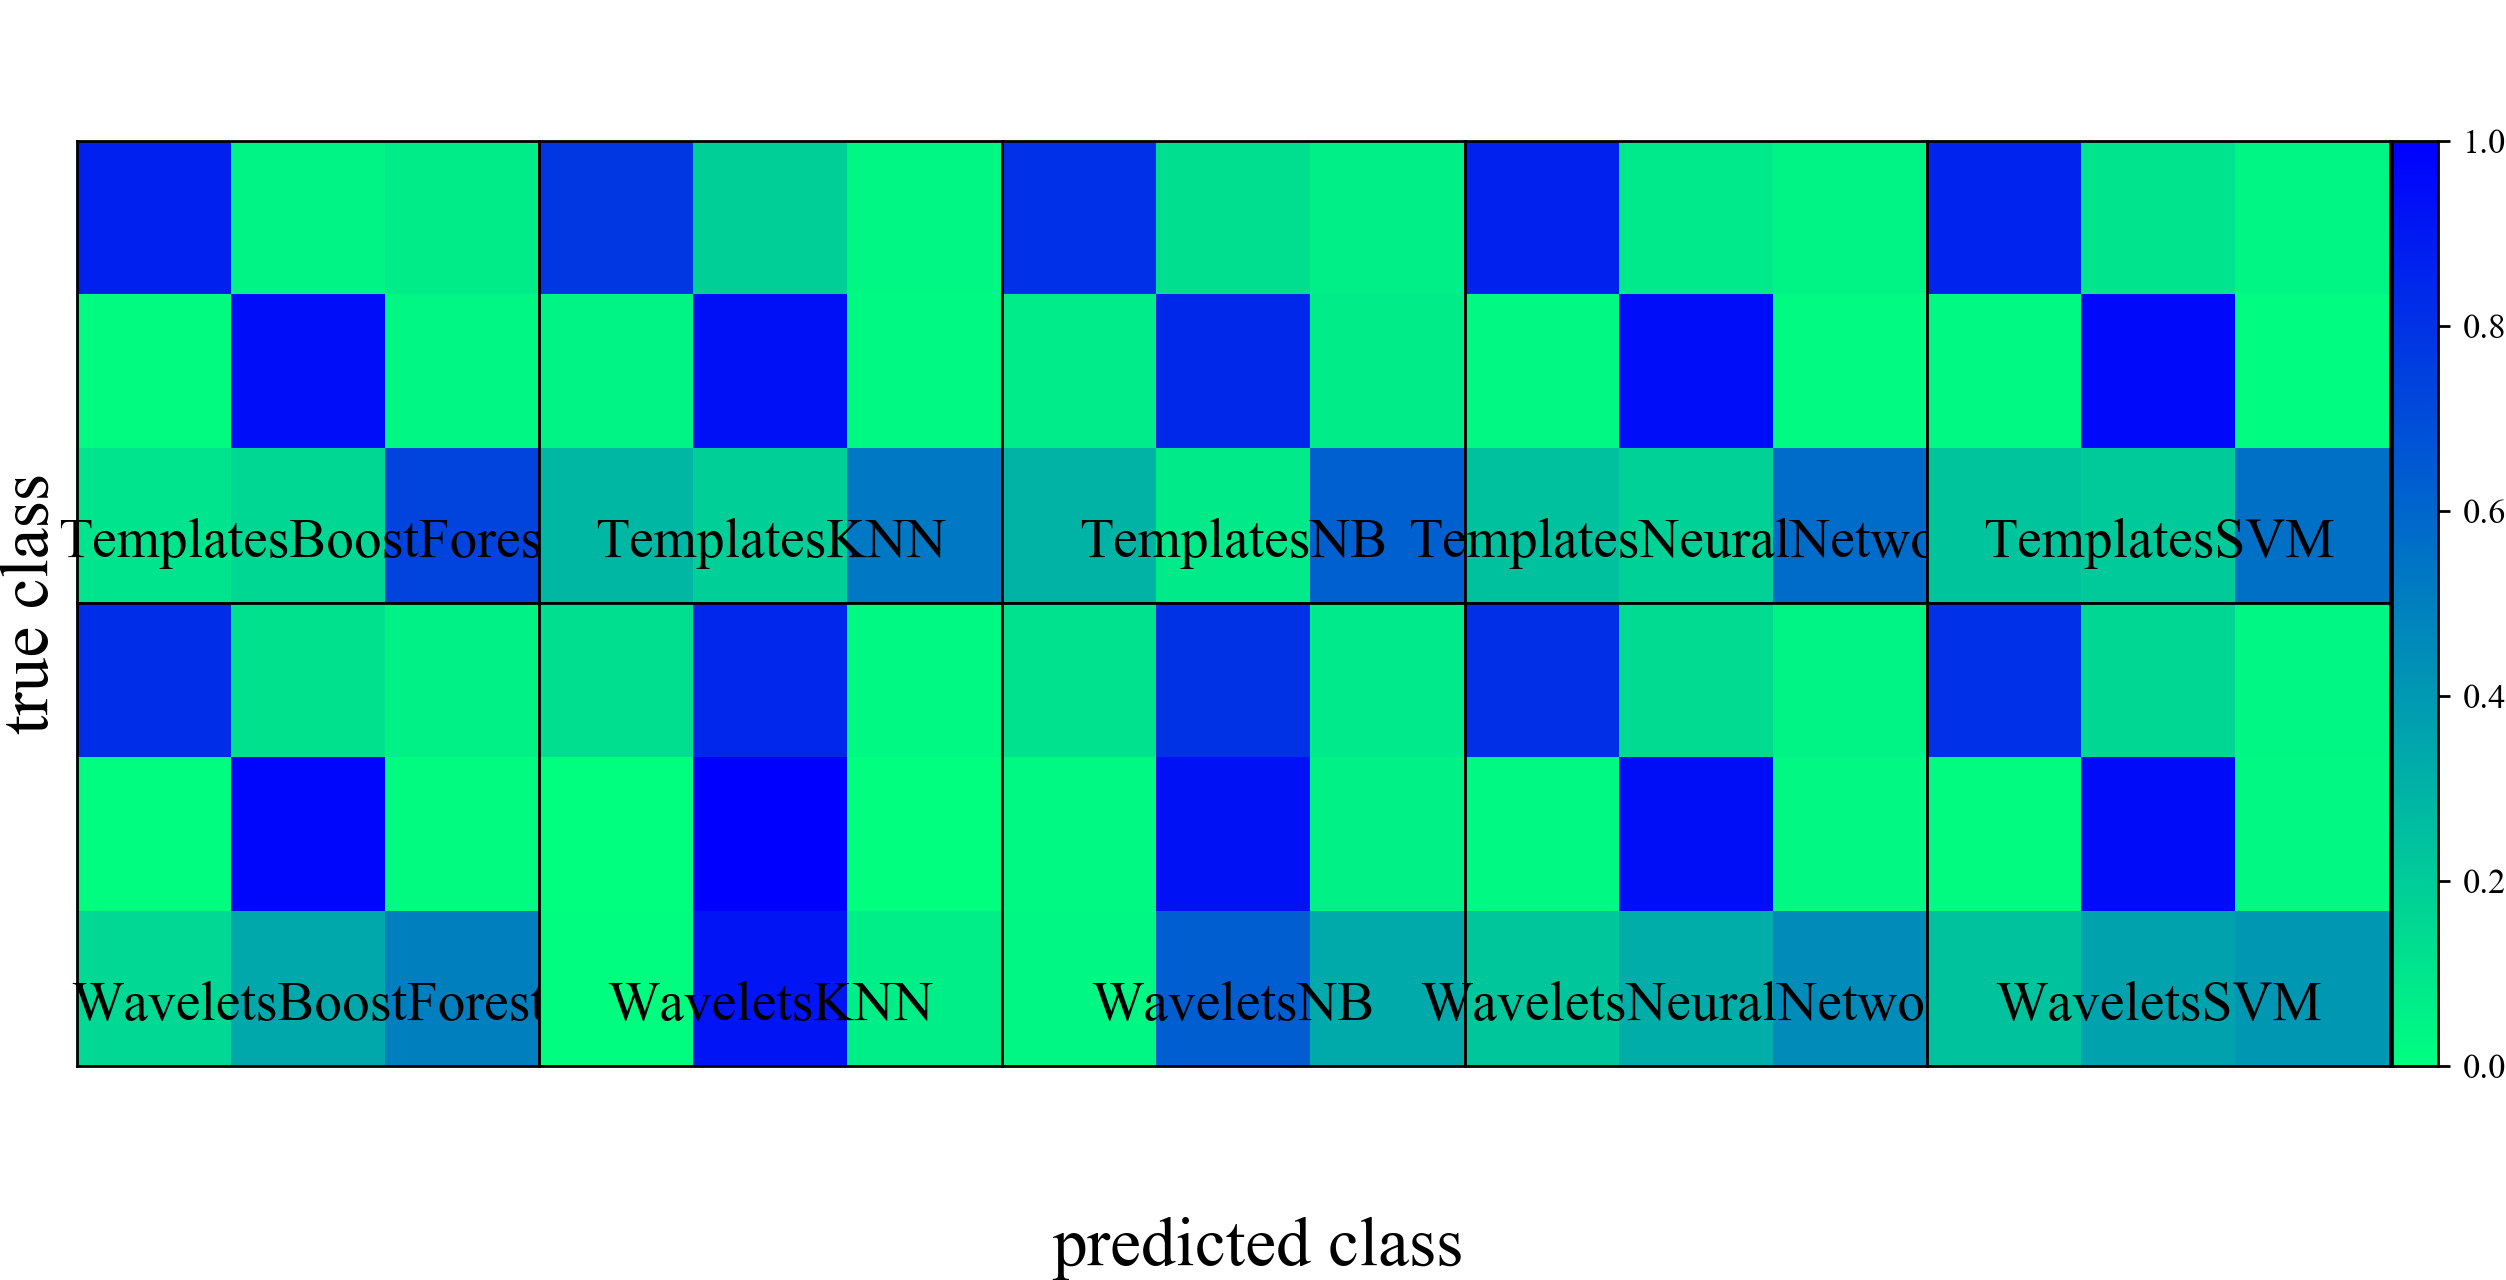
\includegraphics[width=\textwidth]{./fig/all_snphotcc_cm.png}
		\caption{SNPhotCC confusion matrices; note that the KNN classifiers suffer from the cruise control systematic, }
		\label{fig:snphotcc_cm}
	\end{center}
\end{figure*}



% \subsubsection{Unknown dataset}
% \label{sec:mystery}
%
% \begin{figure*}
% 	\begin{center}
% 		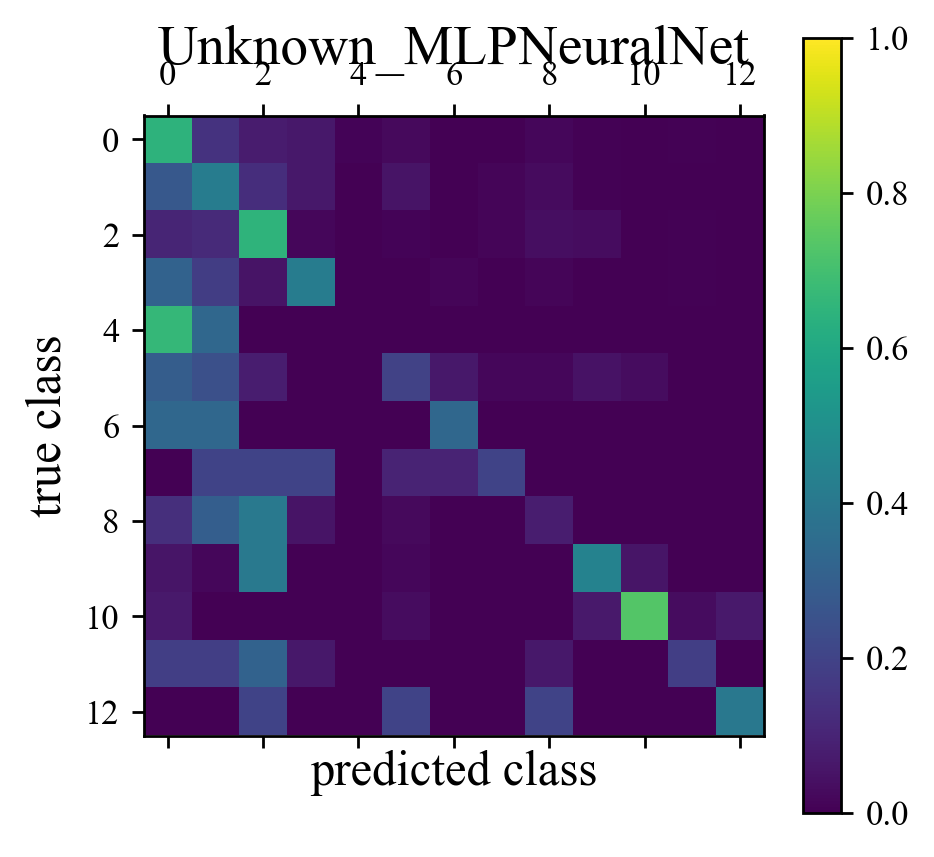
\includegraphics[width=0.3\textwidth]{./fig/Unknown_MLPNeuralNet_cm.png}
% 		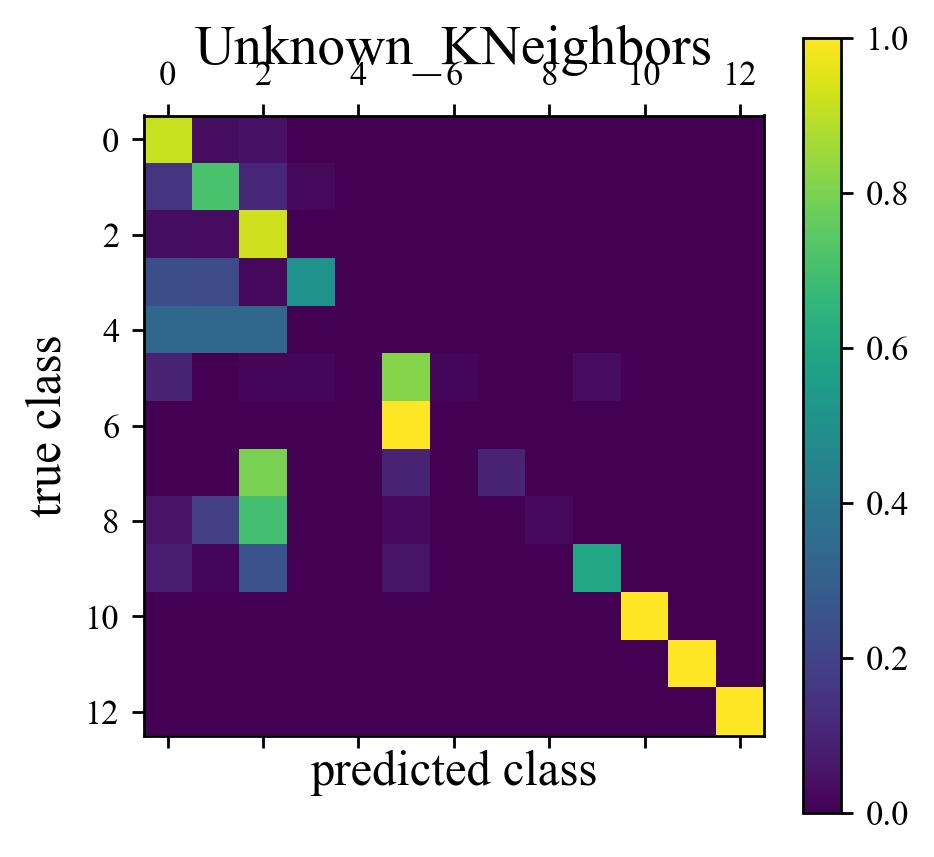
\includegraphics[width=0.3\textwidth]{./fig/Unknown_KNeighbors_cm.png}
% 		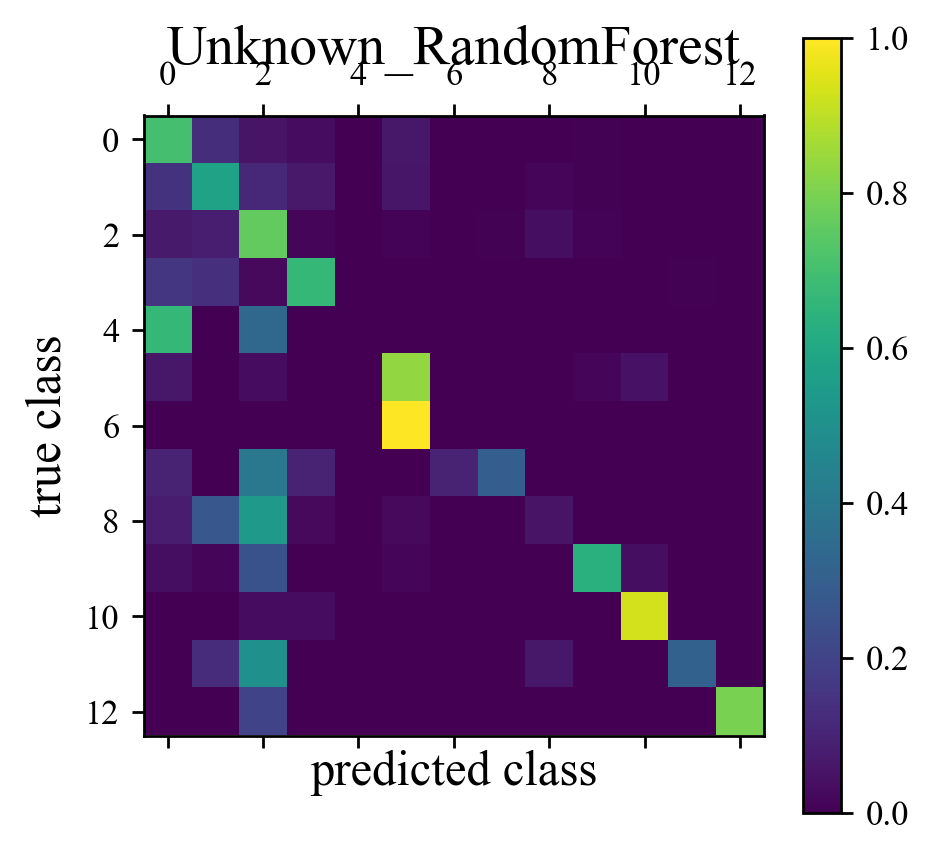
\includegraphics[width=0.3\textwidth]{./fig/Unknown_RandomForest_cm.png}
% 		\caption{}
% 		\label{fig:unknown_cm}
% 	\end{center}
% \end{figure*}
